\documentclass{llncs}

\usepackage{graphicx}
\usepackage{booktabs}
\usepackage{amsmath,amssymb}
\usepackage{cite}
\usepackage{algorithm}
\usepackage{algorithmic}
\usepackage{url}
\usepackage{subfig}
\usepackage{microtype}
\usepackage{xcolor}

\usepackage{hyperref}
\hypersetup{
    colorlinks=true,
    linkcolor=blue,
    citecolor=blue,
    urlcolor=blue
}

% Float control parameters to optimize LNCS page flow
\renewcommand{\topfraction}{0.95}
\renewcommand{\bottomfraction}{0.95}
\renewcommand{\textfraction}{0.05}
\renewcommand{\floatpagefraction}{0.85}
\setcounter{topnumber}{4}
\setcounter{bottomnumber}{4}
\setcounter{totalnumber}{6}
\setlength{\floatsep}{4pt plus 2pt minus 1pt}
\setlength{\textfloatsep}{6pt plus 2pt minus 1pt}
\setlength{\intextsep}{4pt plus 2pt minus 1pt}
\setlength{\abovedisplayskip}{3pt plus 1pt minus 1pt}
\setlength{\belowdisplayskip}{3pt plus 1pt minus 1pt}
\setlength{\abovedisplayshortskip}{1pt plus 1pt minus 1pt}
\setlength{\belowdisplayshortskip}{1pt plus 1pt minus 1pt}

% Compact bibliography formatting for LNCS 12-page camera-ready fit
\let\origthebibliography\thebibliography
\let\endorigthebibliography\endthebibliography
\renewenvironment{thebibliography}[1]{%
  \begin{origthebibliography}{#1}%
    \setlength{\itemsep}{-2.6pt plus 0.2pt}%
    \setlength{\parskip}{0pt}%
    \footnotesize\sloppy
}{%
  \end{origthebibliography}%
}

\begin{document}

\title{A Drift-Aware Explainable Federated Learning Framework for Personalized ICU Sepsis Prediction}

\author{Sheela Akshar Sakhi \and Ramya G R \and S Vandhana \and Hasini Reddy M \and Kousik Sarma Lakkaraju \and Haswitha K \and V Chakravarthy}
\authorrunning{S. A. Sakhi et al.}

\institute{Department of Computer Science and Engineering, Amrita School of Computing, \\
Amrita Vishwa Vidyapeetham, Coimbatore, India \\
\email{cb.sc.u4cse23547@cb.students.amrita.edu, gr\_ramya@cb.amrita.edu, s\_vandhana@cb.amrita.edu, cb.sc.u4cse23529@cb.students.amrita.edu, cb.sc.u4cse23761@cb.students.amrita.edu, cb.sc.u4cse23363@cb.students.amrita.edu, cb.sc.u4cse23753@cb.students.amrita.edu}}

\maketitle
\begin{abstract}
Early sepsis detection in Intensive Care Units (ICUs) is vital to prevent septic shock and mortality, yet decentralized healthcare models face non-IID institutional heterogeneity, temporal concept drift, severe class imbalance ($2.58\%$ positive windows), and limited transparency. We present the Federated Personalized Drift-Aware Attention Framework (FPDAF), unifying (1) Adaptive Divergence-Weighted CUSUM (AD-CUSUM) combining validation-loss residuals, zero-label prediction divergence, gradient-variance damping, and dynamic slack; (2) Dynamic Dual-Phase Saliency and Entropy-Regularized Personalization (DDP-ERP) fusing multi-head temporal and vital co-dependence attention under functional distillation; and (3) Client-Side Selective Personalization (CSSP), which freezes shared backbones and omits backbone synchronization strictly upon detected drift. Across three random seeds on $102{,}994$ held-out windows ($6{,}050$ patient-disjoint encounters) from PhysioNet 2019 across three simulated clients, FPDAF-v2 attains $0.8107\pm 0.0013$ AUROC and $0.1122\pm 0.0021$ AUPRC ($4.35\times$ random prevalence), surpassing Centralized BiLSTM, FedAvg, FedProx, Ditto, and FPDAF-v1. At the validation F1-optimal threshold ($\tau=0.49$), FPDAF-v2 reaches $14.37\pm 0.26\%$ precision, $29.86\pm 0.80\%$ recall, $0.1940\pm 0.0041$ F1-score, and $95.29\pm 0.03\%$ specificity ($5.42$ alerts/100 windows on seed~42). Split-weight retention reduces 10-round communication from $56.43$~MB to $54.37$~MB ($-1.81$~MB per CSSP drift round), while Integrated Gradients ($n=500$) and constrained sensitivity analysis provide non-causal bedside inspection.

\keywords{Federated Learning, Personalized Federated Learning, Sepsis Prediction, Concept Drift, Temporal Attention, Explainable AI.}
\end{abstract}

\section{Introduction}

Sepsis is life-threatening organ dysfunction caused by a dysregulated host response to infection~\cite{21}, where delayed ICU recognition increases mortality and motivates early-intervention bundles~\cite{22}. Since prodromal features (tachycardia, hypotension, tachypnea, hypoxemia) coincide with non-infective illnesses~\cite{17,22}, automated sequential early warning system based on multivariate vitals and laboratory streams would facilitate clinical monitoring~\cite{5,23}. Yet, implementation of such systems encounters three interlinked obstacles: (1) \textbf{Patient Confidentiality:} legal impediments impede direct EHR centralization~\cite{6}, therefore prompting Federated Learning (FL)~\cite{15}; (2) \textbf{Non-IID data heterogeneity and concept drift:} hospital-based demographic differences and evolving clinical acuity per stay undermine static global models~\cite{2,7,16,25}; and (3) \textbf{Alarm burden and interpretability:} low prevalence of severe sepsis leads to alert fatigue due to lack of transparency concerning precision/precision-recall trade-offs and non-causal attributions~\cite{10,24}.

This work proposes the Federated Personalized Drift-Aware Attention Framework (FPDAF) with four key contributions:
\begin{enumerate}\setlength{\itemsep}{1pt}\setlength{\parskip}{0pt}
    \item \textbf{AD-CUSUM Drift Detection:} Combines label-lagged validation-loss residuals, zero-label Jensen--Shannon prediction divergence ($D_{\mathrm{JSD}}$), inverse head-gradient-variance damping, and dispersion slack to separate true shift from minority-class noise.
    \item \textbf{DDP-ERP Dual-Phase Personalization:} Unites multi-head temporal self-attention with inter-variable vital co-dependence attention under functional KL distillation and cosine representation alignment on unconstrained private classification heads.
    \item \textbf{Reconciled CSSP Adaptation:} Jointly trains and synchronizes shared backbones during stationary periods ($S_r \le H$), and exclusively upon detected drift ($S_r > H$) freezes shared backbones, skips backbone server communication, and fine-tunes only local classification heads ($E_{\mathrm{drift}}=5$ epochs).
    \item \textbf{Audited Multi-Seed \& Drift Evaluation:} Establishes strictly patient-disjoint multi-seed benchmarks, precision--recall and threshold calibration, patient-cluster bootstrap CIs, chronological late-ICU drift sensitivity, cohort Integrated Gradients stability~\cite{24}, and constrained counterfactual sensitivity over simulated clients~\cite{23}.
\end{enumerate}

The remainder of this paper covers Related Work (Section~2), Methodology (Section~3), Experimental Setup (Section~4), Empirical Results (Section~5), Explainability and Efficiency (Section~6), Discussion and Limitations (Section~7), and Conclusion (Section~8).

\section{Related Work}

FL helps achieve decentralized learning on EHR data without aggregating raw EHRs centrally~\cite{15}, with FedProx~\cite{25} using proximal regularization for client drift while ensuring privacy-preserving healthcare and FL on time series~\cite{1,5,6,13,14,16,17,18,20,23}. Heterogeneous hospitals require FL to be personalized by using techniques like personalization in FL~\cite{3}, ditto learning~\cite{26}, hierarchical re-weighting~\cite{4}, gradient correction with self-distillation (FedDGC-PSD)~\cite{12}, and personalized forecasting~\cite{19}. In order to deal with temporal distribution changes, distributed drift clustering~\cite{2} and monitored CUSUM/ADWIN adaptation~\cite{7} detect distribution changes sequentially, but suffer from the overhead of multiple branches or excessive false alarms in case of variance in minority class. Interpretability research in CL includes saliency maps~\cite{9}, integrated gradients~\cite{24}, time series interpretation benchmarks~\cite{10}, federated XAI~\cite{8}, and sepsis prediction~\cite{11}.

In contrast to previous drift-aware and PFL approaches~\cite{2,3,7,25,26} which consider adaptation, communication reduction, and interpretability independently, the FPDAF approach considers three interlinked strategies: (i) the AD-CUSUM strategy enhances the validation-loss residual with an unlabeled prediction divergence ($D_{\mathrm{JSD}}$) and inverse gradient variance damping; (ii) the DDP-ERP strategy utilizes dual temporal-vital attention and KL and cosine embedding distillation without penalizing the private heads; and (iii) CSSP freezes the shared backbones and blocks the backbone transmission strictly during the drift period.

\section{Methodology and System Architecture}

FPDAF unifies shared temporal representation learning, unconstrained private classification heads, drift-triggered structural freezing, and clinical explainability (Fig.~\ref{fig:architecture}). Clients execute local preprocessing (Subsystem~1), split-weight inference and local XAI attribution (Subsystem~2), and AD-CUSUM monitoring/CSSP control (Subsystem~3), exchanging only the shared backbone $\theta$ and a $1$-B drift indicator $b_{k,r}\in\{0,1\}$ with the FedAvg server (Subsystem~4). Private heads $\phi_k$, raw EHR trajectories, attribution maps, and validation probes remain strictly local.

\begin{figure}[t]
    \centering
    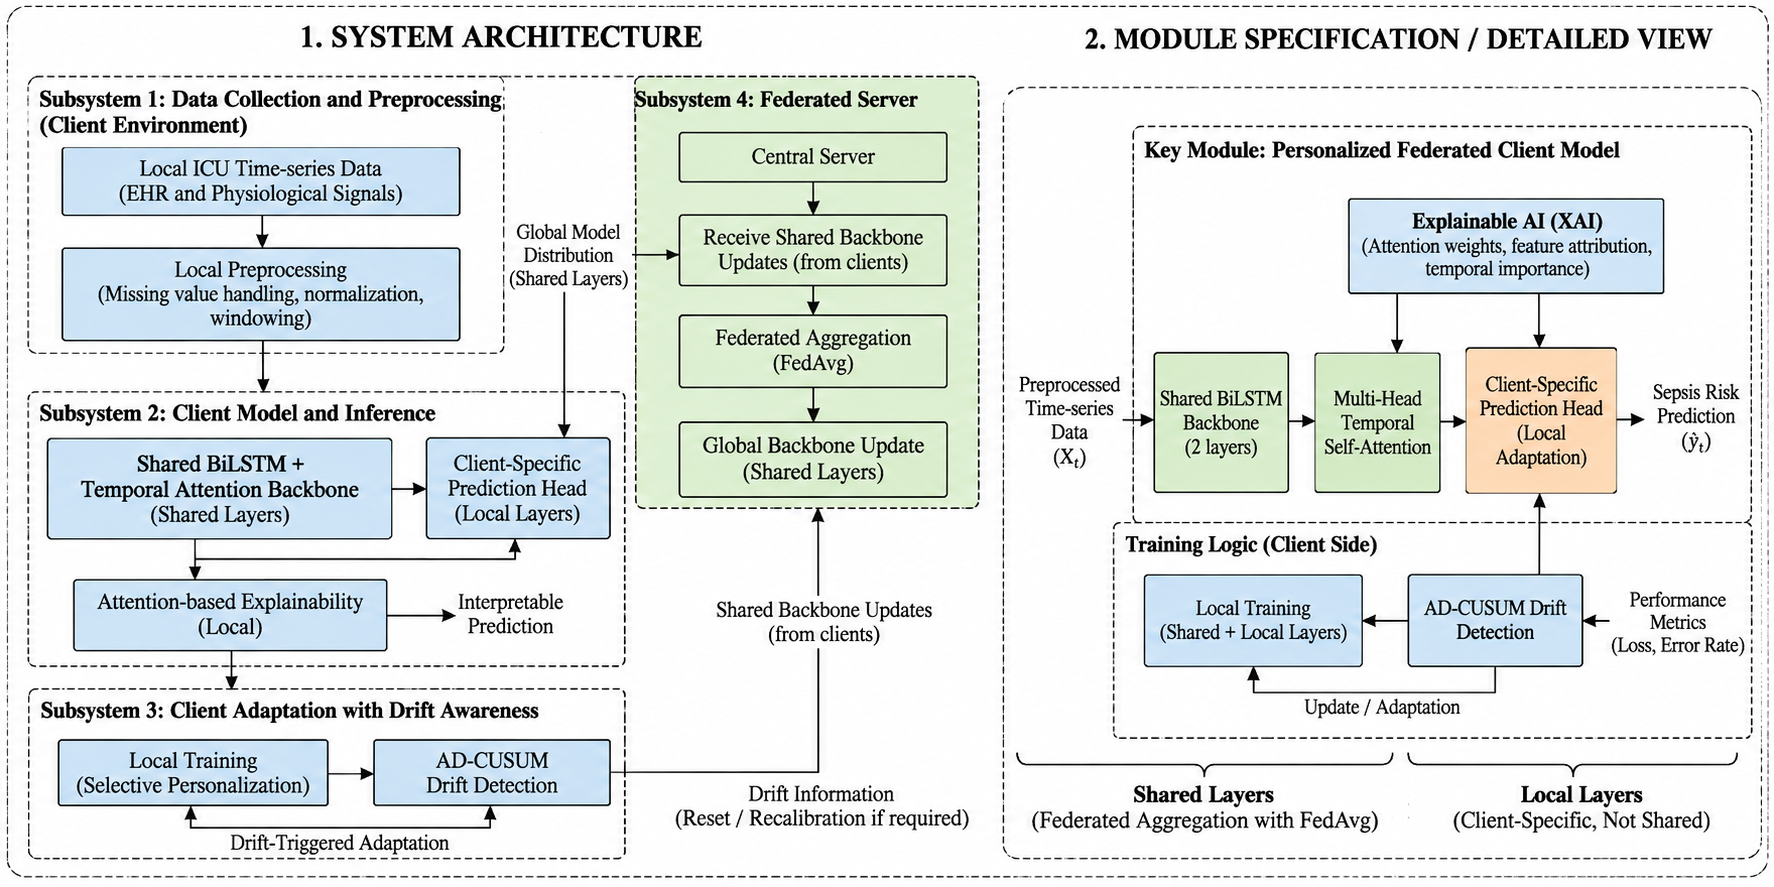
\includegraphics[width=0.79\textwidth]{Fig1.png}
    \caption{Architecture of FPDAF: local preprocessing (Subsystem~1), split-weight inference and XAI (Subsystem~2), AD-CUSUM and CSSP (Subsystem~3), and backbone-only FedAvg aggregation (Subsystem~4; $\phi_k$ and raw data remain strictly local).}
    \label{fig:architecture}
\end{figure}

\subsection{Split-Weight Dual-Phase Attention Architecture}

Let $K=3$ simulated clients hold local datasets $\mathcal{D}_k=\{(X_i^k,y_i^k)\}_{i=1}^{N_k}$ with $X_i^k\in\mathbb{R}^{T\times F}$ ($T=24$~h, $F=40$ features). Each model splits into shared backbone $g_\theta$ and private head $h_{\phi_k}$ (\texttt{128}$\to$\texttt{64}$\to$\texttt{ReLU}$\to$\texttt{Dropout(0.3)}$\to$\texttt{1}; $8{,}321$ params, $35{,}485$~B). A two-layer BiLSTM ($64$ units/direction, dropout $0.3$, output $d=128$) generates hidden states $H=[h_1,\ldots,h_T]\in\mathbb{R}^{T\times d}$.

In \textit{FPDAF-v1}, $g_\theta$ applies $M=4$-head scaled dot-product temporal self-attention ($d_k=d/M=32$):
\begin{equation}
A_m = \mathrm{softmax}\!\left(\frac{(H W_m^Q)(H W_m^K)^{\top}}{\sqrt{d_k}}\right)(H W_m^V), \qquad m=1,\ldots,M,
\end{equation}
concatenating heads $C=[A_1,\ldots,A_M]\in\mathbb{R}^{T\times d}$ (with hourly rows $c_t\in\mathbb{R}^{d}$) and pooling $c_{\mathrm{temp}} = W^O\!\left(\frac{1}{T}\sum_{t=1}^{T} c_t\right)+b^O$ ($227{,}585$ params / $918{,}168$~B total; $\theta$: $219{,}264$ params / $883{,}492$~B). In \textit{FPDAF-v2}, Dual-Phase Cross-Attention fuses $c_{\mathrm{temp}}$ with an inter-variable vital co-dependence pathway over standardized vectors $x_t\in\mathbb{R}^{F}$:
\begin{equation}
u_t = W_v x_t + b_v,\qquad
\gamma_t = \frac{\exp(w_c^{\top} u_t + b_c)}{\sum_{j=1}^{T}\exp(w_c^{\top} u_j + b_c)},\qquad
c_{\mathrm{vital}} = \frac{1}{T}\sum_{t=1}^{T}\gamma_t u_t,
\end{equation}
producing fused embedding $z_k = c_{\mathrm{temp}} + c_{\mathrm{vital}}$ and prediction $\hat{y}_k = \sigma(h_{\phi_k}(z_k))$ ($232{,}962$ params / $941{,}132$~B total; $\theta$: $224{,}641$ params / $906{,}200$~B). Temporal self-attention weights aggregate as $\alpha_t = \frac{1}{MT}\sum_{m=1}^{M}\sum_{j=1}^{T}(A^{\mathrm{attn}}_m)_{j,t}$.

\subsection{Adaptive Divergence-Weighted CUSUM (AD-CUSUM)}

To separate genuine distributional shift from minority-class noise, AD-CUSUM integrates: (i) adjudicated validation-loss residual $(L_{\mathrm{val},r}-\mu_0)$ against stationary baseline $\mu_0$ (evaluated under realistic 1-round clinical label lag $L_{\mathrm{val},r-1}$, zero-lag, and loss-only ablations); (ii) unlabeled prediction Jensen--Shannon divergence across consecutive batches:
\begin{equation}
D_{\mathrm{JSD}}(P_r\|P_{r-1})
=\frac{1}{2}D_{\mathrm{KL}}(P_r\|M)
+\frac{1}{2}D_{\mathrm{KL}}(P_{r-1}\|M),\qquad M=\frac{P_r+P_{r-1}}{2},
\end{equation}
requiring zero ground-truth labels; (iii) head-gradient-variance damping suppressing noisy updates,
\begin{equation}
w_{\mathrm{grad}}^{(r)}=\left[1+\gamma\,\mathrm{Var}\!\left(\|\nabla_{\phi_k}\mathcal{L}\|_2^2\right)\right]^{-1};
\end{equation}
and (iv) dynamic trailing-dispersion slack $\kappa_r = \kappa_0 + \alpha\sigma_{\mathrm{hist},r}$ over the prior five adjudicated losses (with regime baseline $\kappa_0$). The cumulative statistic evolves as
\begin{equation}\label{eq:ad_cusum}
S_r=\max\!\left(0,\,S_{r-1}+w_{\mathrm{grad}}^{(r)}\!\left[(L_{\mathrm{val},r}-\mu_0)+\beta D_{\mathrm{JSD}}^{(r)}-\kappa_r\right]\right).
\end{equation}
Drift triggers when $S_r>H$ (setting drift flag $b_{k,r}\leftarrow 1$ and resetting $S_r\leftarrow 0$). Requiring cumulative excess over $\kappa_r$ rejects isolated spikes, while $H=3.0$ enforces $3\sigma$-style false-alarm control (swept across $H\in[1.5,4.0]$ in Section~5.3), with $\gamma=0.5, \alpha=0.1$ ($\beta=0.15, \kappa_0=0.02$ during 10-round training; $\beta=1.2, \kappa_0=0.05$ during 30-round deployment monitoring).

\subsection{DDP-ERP and Client-Side Selective Personalization (CSSP)}

Whereas FPDAF-v1 pairs single-phase attention and loss-only CUSUM with Euclidean $L_2$ backbone anchoring ($\mathcal{L}_{\mathrm{v1}} = \mathcal{L}_{\mathrm{wBCE}} + \frac{\lambda}{2}\|\theta_k-\theta_{\mathrm{glob}}\|_2^2$), FPDAF-v2 optimizes positive-weighted BCE ($\mathrm{pos\_weight}=8.0$) with functional logit distillation and hyperspherical embedding alignment:
\begin{equation}\label{eq:ddp_erp}
\mathcal{L}_{\mathrm{DDP-ERP}}
=\mathcal{L}_{\mathrm{wBCE}}
+\lambda D_{\mathrm{KL}}(P_k\|P_{\mathrm{glob}})
+\eta\left(1-\cos(z_k,z_{\mathrm{glob}})\right),
\end{equation}
where $\lambda=0.1, \eta=0.05$, freeing $\phi_k$ from weight penalties. Under \textbf{CSSP} (Algorithm~\ref{alg:fpdaf}), during stable rounds ($b_{k,r-1}=0$) clients synchronize $\theta$, retain $\phi_k$, jointly update $(\theta_k,\phi_k)$, and upload $\theta_k$ ($906{,}200$~B); when prior-round AD-CUSUM triggers drift ($b_{k,r-1}=1$, i.e., $S_{r-1}$ exceeded $H$ prior to reset), client $k$ freezes $\theta_k$, skips backbone download/upload (sending only the $1$-B flag $b_{k,r-1}=1$ so FedAvg excludes $\theta_k$ and renormalizes over synchronizing clients), and fine-tunes only $\phi_k$ for $E_{\mathrm{drift}}=5$ local epochs, saving $1.81$~MB per client drift round.

\begin{algorithm}[t]
\caption{FPDAF-v2 Training, AD-CUSUM Monitoring, and CSSP Adaptation}
\label{alg:fpdaf}
\begin{algorithmic}[1]
\scriptsize
\STATE \textbf{Input:} Clients $k \in \{0,1,2\}$, initial shared $\theta^{(0)}$, private heads $\phi_k^{(0)}$, $b_{k,0}\leftarrow 0$, $S_{k,0}\leftarrow 0$, threshold $H=3.0$.
\FOR{round $r = 1, \dots, R$}
  \FOR{each client $k$ in parallel}
    \IF{$b_{k,r-1} = 1$ (Drift Triggered)}
      \STATE Freeze $\theta_k$; transmit 1-B flag $b_{k,r-1}=1$ (skip backbone DL/UL); fine-tune only $\phi_k$ for $E_{\mathrm{drift}}=5$ epochs under $\mathcal{L}_{\mathrm{wBCE}}$; reset $b_{k,r}\leftarrow 0$.
    \ELSE
      \STATE Receive $\theta^{(r-1)}$, retain $\phi_k$, update $(\theta_k,\phi_k)$ for $1$ epoch via~\eqref{eq:ddp_erp}; upload $\theta_k^{(r)}$ ($906{,}200$~B).
      \STATE Update $S_{k,r}$ via~\eqref{eq:ad_cusum} using $D_{\mathrm{JSD}}^{(r)}, w_{\mathrm{grad}}^{(r)}, \kappa_r$ and $L_{\mathrm{val}}$; if $S_{k,r} > H$ then $b_{k,r}\leftarrow 1, S_{k,r} \leftarrow 0$ else $b_{k,r}\leftarrow 0$.
    \ENDIF
  \ENDFOR
  \STATE $\mathcal{A}_r \leftarrow \{k : b_{k,r-1}=0\}$; if $\mathcal{A}_r \neq \emptyset$ then $\theta^{(r)} \leftarrow \sum_{k\in\mathcal{A}_r}\frac{N_k}{\sum_{j\in\mathcal{A}_r} N_j}\theta_k^{(r)}$ else $\theta^{(r)} \leftarrow \theta^{(r-1)}$.
\ENDFOR
\end{algorithmic}
\end{algorithm}

\section{Experimental Setup and Preprocessing}

\subsection{Dataset, Patient-Disjoint Splitting, and Six-Hour Target}

Experiments use the public PhysioNet/CinC Challenge 2019 sepsis cohort~\cite{23} comprising $40{,}327$ hourly multivariate ICU stays across two hospital systems (Hospital~A: $20{,}336$; Hospital~B: $19{,}991$) and $F=40$ physiological, laboratory, and demographic variables. To eliminate sequence overlap across splits, patients are stratified by hospital and randomly partitioned at the \textbf{patient level} ($70\%/15\%/15\%$, seed~$42$) \emph{before} scaling or windowing: Train ($28{,}228$ patients; $2{,}114$ sepsis; $477{,}669$ windows, $2.62\%$ pos.), Validation ($6{,}049$ patients; $396$ sepsis; $104{,}038$ windows, $2.35\%$ pos.), and Test ($6{,}050$ patients; $421$ sepsis; $102{,}994$ windows, $2.58\%$ pos.; $2{,}655$ pos., $100{,}339$ neg.), with verified zero pairwise patient overlap ($0/0/0$).

Following PhysioNet 2019 labeling~\cite{23}, positive patients have $\mathrm{SepsisLabel}=1$ from six hours before clinical onset ($t \ge t_{\mathrm{onset}}-6$) through all recorded post-onset ICU hours. Rolling $24$-h windows $X[t:t+24]\in\mathbb{R}^{24\times 40}$ receive the label at window endpoint $t+23$; shorter stays ($T<24$~h) are left-zero-padded into one terminal sequence. Of $2{,}655$ positive test windows, $1{,}999$ lie within the pre-onset/onset horizon and $656$ follow onset (Section~5.1).

\subsection{Preprocessing}

To ensure no cross-patient contamination, patient-wise splitting is applied before any imputations, normalization, and windowing. Missing values in each hospitalization are imputed through causal forward fill (\texttt{ffill}) and admissions fill (for the initial sparse period before measurements) using median of training split (with forced fallback in the new imputation module) and zero-fill for missing variables. Continuous features are scaled using only training split statistics through \texttt{StandardScaler}:
\begin{equation}\label{eq:std}
z=\frac{x-\mu_{\mathrm{train}}}{\sigma_{\mathrm{train}}}.
\end{equation}
Validation and test transforms reuse $(\mu_{\mathrm{train}},\sigma_{\mathrm{train}})$ without re-fitting, producing $24\times 40$ tensors with zero missing or infinite entries.

\subsection{Simulated Client Partitioning, Protocol, and Drift Setup}

All three clients are simulated from the PhysioNet 2019 cohort~\cite{23}:
\textbf{Client~0 (Hospital~A, Age $<60$)} holds $92{,}613$ train ($3.24\%$ pos., $5{,}705$ patients, age $46.44\pm10.89$), $19{,}953$ val ($2.96\%$), and $19{,}530$ test ($2.89\%$, $1{,}219$ patients) windows; \textbf{Client~1 (Hospital~A, Age $\ge 60$)} holds $151{,}916$ train ($3.09\%$ pos., $8{,}530$ patients, age $73.61\pm7.78$), $33{,}376$ val ($2.77\%$), and $32{,}667$ test ($3.25\%$, $1{,}832$ patients) windows; and \textbf{Client~2 (Hospital~B)} holds $233{,}140$ train ($2.07\%$ pos., $13{,}993$ patients, age $61.11\pm16.49$), $50{,}709$ val ($1.83\%$), and $50{,}797$ test ($2.03\%$, $2{,}999$ patients) windows. Standardized Wasserstein-1 distances confirm substantial non-IID heterogeneity: Age $W_1(0,1)=1.6625$, $W_1(0,2)=0.8980$, $W_1(1,2)=0.7939$; MAP $W_1(1,2)=0.5227$; HR $W_1(0,1)=0.2848$; WBC $W_1(1,2)=0.2406$; Lactate $W_1(0,2)=0.2160$.

Every benchmark and ablation trains on identical splits for $10$ rounds using a stratified budget of $15{,}000$ training windows/client ($45{,}000$/seed), $1$ local training epoch/stable round ($E_{\mathrm{drift}}=5$ on drift), batch size $256$, and the \textbf{Adam optimizer} ($\mathrm{lr}=5\times 10^{-4}$, weight decay $5\times 10^{-4}$, grad clip $1.0$, $\mathrm{pos\_weight}=8.0$) across seeds $\{42,123,999\}$. Model selection uses full validation AUROC, thresholds calibrate solely on validation probabilities, and communication bytes sum serialized \texttt{state\_dict} transfers plus $1$-B CSSP flags in decimal megabytes ($1\text{ MB}=10^6\text{ B}$; zero probe/XAI network traffic). Chronological drift runs over a 30-round test stream ($500$ windows/round, $5$ Monte Carlo orderings): rounds $r=1\dots 10$ draw early/mid-ICU stays ($\mathrm{ICULOS}\le 48$~h, Client~1 $1.59\%$ pos.), transitioning at $r^*=11$ to late-ICU stays ($\mathrm{ICULOS}>60$~h, $13.37\%$ pos., $8.4\times$ shift) with stationary Client~0 ($\mathrm{ICULOS}\le 48$~h) as negative control, evaluated under 1-round clinical label lag vs.\ zero-lag and loss-only CUSUM across $H\in\{1.5,\dots,4.0\}$.


\section{Empirical Evaluation and Results}

\subsection{Benchmark, Ablation, and Pre-/Post-Onset Performance}

Table~\ref{tab:results} summarizes the three-seed evaluation ($\{42,123,999\}$) across identical splits on all $N=102{,}994$ held-out test windows ($2{,}655$ pos., $100{,}339$ neg.; $6{,}050$ patients) at $\tau=0.50$. Under $2.58\%$ prevalence, FPDAF-v2 attains the top AUROC ($0.8107\pm 0.0013$; Fig.~\ref{fig:combined}(a)), AUPRC ($0.1122\pm 0.0021$; $4.35\times$ random prevalence, Fig.~\ref{fig:pr_curves}), precision ($14.45\pm 0.32\%$), and F1-score ($0.1932\pm 0.0036$), with $6.5\times$ lower cross-seed AUROC SD ($\pm 0.0013$) than FedAvg ($\pm 0.0084$) and Centralized BiLSTM ($\pm 0.0094$). At validation F1-optimal $\tau_{\mathrm{val}}=0.49$, FPDAF-v2 reaches $14.37\pm 0.26\%$ precision, $29.86\pm 0.80\%$ recall, $95.29\pm 0.03\%$ specificity, and $0.1940\pm 0.0041$ F1 (Seed~42: $\mathrm{TP}=820, \mathrm{FP}=4{,}763, \mathrm{TN}=95{,}576, \mathrm{FN}=1{,}835$).

In Part~B ablations, removing personalization drops AUROC to $0.7979$ and AUPRC to $0.0989$; removing attention increases seed variance ($2.5\times$) and reduces AUPRC ($0.1111$); and removing AD-CUSUM on stationary 10-round training yields identical trajectories ($0.0\%$ stationary false-alarm penalty before chronological shift, Section~5.3). On Seed~42 pre- vs.\ post-onset windows, FPDAF-v2 attains $27.51\%$ pre-onset and $34.45\%$ post-onset recall at $\tau=0.50$ ($72.34\%$ and $84.91\%$ at Youden $\tau=0.21$), detecting $263/421$ septic patients at median $6.0$~h lead time (mean $5.11\pm 1.60$~h).

\begin{table}[t]
\centering
\caption{Three-seed comparative benchmark and ablations on the full held-out PhysioNet 2019 test partition ($N=102{,}994$ windows: $2{,}655$ positive, $100{,}339$ negative; $6{,}050$ patients) evaluated at $\tau=0.50$. Means $\pm$ SD across seeds $\{42,123,999\}$ and Seed-42 confusion counts.}
\label{tab:results}
\resizebox{\textwidth}{!}{%
\begin{tabular}{lccccccccr}
\toprule
\textbf{Configuration} & \textbf{AUROC} & \textbf{AUPRC} & \textbf{Acc. (\%)} & \textbf{Prec. (\%)} & \textbf{Rec. (\%)} & \textbf{Spec. (\%)} & \textbf{F1} & \textbf{Comm.} & \textbf{Seed-42 (TP/FP/TN/FN)} \\
\midrule
\multicolumn{10}{l}{\textit{Part A: Comparative Benchmarks (10 Federated Rounds / 15k Windows per Client)}} \\
\midrule
Centralized BiLSTM & $0.8008{\pm}0.0094$ & $0.1013{\pm}0.0039$ & $89.54{\pm}0.75$ & $11.23{\pm}0.32$ & $44.17{\pm}2.95$ & $90.74{\pm}0.85$ & $0.1789{\pm}0.0032$ & -- & 1,282 / 10,484 / 89,855 / 1,373 \\
FedAvg & $0.8032{\pm}0.0084$ & $0.1012{\pm}0.0039$ & $89.88{\pm}0.08$ & $11.04{\pm}0.31$ & $41.51{\pm}1.88$ & $91.16{\pm}0.13$ & $0.1744{\pm}0.0055$ & 39.23 MB & 1,113 / 8,953 / 91,386 / 1,542 \\
FedProx & $0.8004{\pm}0.0084$ & $0.1019{\pm}0.0072$ & $89.85{\pm}0.10$ & $10.99{\pm}0.27$ & $41.41{\pm}1.80$ & $91.13{\pm}0.15$ & $0.1737{\pm}0.0050$ & 39.23 MB & 1,108 / 8,971 / 91,368 / 1,547 \\
Personalized FL (Ditto) & $0.8067{\pm}0.0027$ & $0.1089{\pm}0.0023$ & $90.11{\pm}0.19$ & $11.83{\pm}0.33$ & $43.92{\pm}1.18$ & $91.34{\pm}0.20$ & $0.1864{\pm}0.0049$ & 39.23 MB & 1,210 / 8,705 / 91,634 / 1,445 \\
FPDAF-v1 & $0.8075{\pm}0.0011$ & $0.1117{\pm}0.0021$ & $93.91{\pm}0.44$ & $14.39{\pm}0.80$ & $27.33{\pm}1.19$ & $95.67{\pm}0.49$ & $0.1881{\pm}0.0043$ & 53.01 MB & 694 / 3,910 / 96,429 / 1,961 \\
\textbf{FPDAF-v2} & $\mathbf{0.8107{\pm}0.0013}$ & $\mathbf{0.1122{\pm}0.0021}$ & $93.72{\pm}0.10$ & $\mathbf{14.45{\pm}0.32}$ & $29.14{\pm}0.54$ & $95.43{\pm}0.10$ & $\mathbf{0.1932{\pm}0.0036}$ & 54.37 MB & 776 / 4,444 / 95,895 / 1,879 \\
\midrule
\multicolumn{10}{l}{\textit{Part B: Component Ablation (Identical Partitions and Seeds)}} \\
\midrule
FPDAF w/o AD-CUSUM & $0.8107{\pm}0.0013$ & $0.1122{\pm}0.0021$ & $93.72{\pm}0.10$ & $14.45{\pm}0.32$ & $29.14{\pm}0.54$ & $95.43{\pm}0.10$ & $0.1932{\pm}0.0036$ & 54.37 MB & 776 / 4,444 / 95,895 / 1,879 \\
FPDAF w/o Attention & $0.8107{\pm}0.0033$ & $0.1111{\pm}0.0018$ & $91.94{\pm}0.87$ & $13.00{\pm}0.98$ & $36.81{\pm}2.49$ & $93.40{\pm}0.96$ & $0.1914{\pm}0.0068$ & 37.17 MB & 886 / 5,275 / 95,064 / 1,769 \\
FPDAF w/o Personaliz. & $0.7979{\pm}0.0022$ & $0.0989{\pm}0.0048$ & $88.12{\pm}0.37$ & $10.43{\pm}0.20$ & $47.52{\pm}2.06$ & $89.20{\pm}0.43$ & $0.1710{\pm}0.0035$ & 56.43 MB & 1,272 / 10,620 / 89,719 / 1,383 \\
\bottomrule
\end{tabular}}
\end{table}

\subsection{Cluster Bootstrap Uncertainty and Clinical Operating Modes}

Because hourly windows within an ICU encounter are correlated, we perform $B=2{,}000$ patient-cluster bootstrap replicates resampling the $M=6{,}050$ test patients (Seed~42; Fig.~\ref{fig:combined}(a) and Fig.~\ref{fig:pr_curves}). FPDAF-v2 achieves AUROC $0.8121$ ($95\%$ CI $[0.7909, 0.8333]$) and AUPRC $0.1151$ ($[0.1060, 0.1337]$), exceeding Centralized BiLSTM ($0.7979$ $[0.7737, 0.8203]$, paired $\Delta=+0.0143$ $[+0.0021, +0.0270]$, $p=0.0250$), FedProx ($0.8058$, $\Delta=+0.0063$, $p=0.1590$), Ditto ($0.8066$, $\Delta=+0.0055$, $p=0.1660$), FPDAF-v1 ($0.8088$, $\Delta=+0.0033$, $p=0.3320$), and FedAvg ($0.8094$, $\Delta=+0.0028$, $p=0.5360$). Table~\ref{tab:thresholds} reports Seed-42 FPDAF-v2 performance with Wilson $95\%$ CIs across five validation-calibrated thresholds, highlighting the alert-burden trade-off from sensitive screening ($\tau=0.15$: $80.98\%$ recall, $35.83$ alerts/100w) to F1-optimal ($0.49$: $14.69\%$ precision, $95.25\%$ specificity, $5.42$ alerts/100w) and high-specificity rule-in ($\tau=0.55$: $98.33\%$ specificity, $17.50\%$ precision, $1.97$ alerts/100w).

\begin{table}[t]
\centering
\caption{Clinical operating-point analysis of FPDAF-v2 on held-out test windows ($N=102{,}994$, Seed~42). All non-default thresholds calibrated strictly on validation probabilities.}
\label{tab:thresholds}
\resizebox{\textwidth}{!}{%
\begin{tabular}{lccccccc}
\toprule
\textbf{Operating Mode} & $\tau$ & \textbf{Acc. (\%)} & \textbf{Prec. (\%)} & \textbf{Sensitivity (95\% CI)} & \textbf{Specificity (95\% CI)} & \textbf{F1} & \textbf{Alerts / 100w} \\
\midrule
Early Screening ($\ge 80\%$ val sens.) & 0.15 & 65.77 & 5.83 & 80.98 (79.44--82.43) & 65.36 (65.07--65.66) & 0.1087 & 35.83 \\
Youden Optimal (val) & 0.21 & 73.95 & 7.11 & 75.44 (73.77--77.04) & 73.91 (73.64--74.18) & 0.1299 & 27.36 \\
F1-Optimal (val) & 0.49 & 93.59 & 14.69 & 30.89 (29.16--32.67) & 95.25 (95.12--95.38) & 0.1991 & 5.42 \\
Default Threshold & 0.50 & 93.86 & 14.87 & 29.23 (27.53--30.99) & 95.57 (95.44--95.70) & 0.1971 & 5.07 \\
High-Spec. Rule-In ($\ge 98\%$ val spec.) & 0.55 & 96.14 & 17.50 & 13.37 (12.13--14.72) & 98.33 (98.25--98.41) & 0.1516 & 1.97 \\
\bottomrule
\end{tabular}}
\end{table}

\subsection{Chronological Drift Sensitivity and Post-Drift CSSP Adaptation}

Table~\ref{tab:drift} and Fig.~\ref{fig:combined}(b) evaluate AD-CUSUM across thresholds $H\in[1.5,4.0]$ on the 30-round chronological late-ICU shift protocol ($r^*=11$; $1.59\%\to 13.37\%$ prevalence). Both AD-CUSUM (under 1-round clinical label lag and ideal 0-round lag) and Loss-Only CUSUM achieve $100\%$ shift detection with $0.0\%$ pre-change FAR ($r=1\dots 10$) and $0.0\%$ stationary control-client FAR (Client~0 across 30 rounds). Under 0-round lag, AD-CUSUM detects drift $1.0$ round faster than 1-round lagged monitors ($2.60$ vs.\ $3.60$ rounds at $H=3.0$) thanks to unlabeled $D_{\mathrm{JSD}}$, and edges out Loss-Only CUSUM even with 1-round lag at $H=2.0$ ($2.60$ vs.\ $2.80$ rounds).

Assessing strictly patient-disjoint post-drift CSSP adaptation (5 local epochs freezing $\theta$) reveals two instructive regimes: under institutional shift (Client~1 head transferred to unseen Hospital~B test patients, $n_{\mathrm{eval}}=25{,}242$), CSSP reduces weighted-BCE loss from $0.4550$ to $0.3322$, cuts Brier calibration error by $63.1\%$ ($0.1038\to 0.0383$), and increases AUROC ($0.8143\to 0.8169$) and AUPRC ($0.0682\to 0.0750$). Conversely, under severe late-ICU prior shift ($\mathrm{ICULOS}>48$~h, $9.48\%$ prevalence, $n_{\mathrm{eval}}=3{,}950$), static \texttt{pos\_weight=8.0} over-weights minority positives and degrades Brier error ($0.2004\to 0.2723$), whereas prior-matched unweighted fine-tuning cuts Brier error by $57.4\%$ ($0.2004\to 0.0853$) though frozen-backbone AUROC dips ($0.6360\to 0.5968$), identifying when unfreezing representation layers is needed alongside head adaptation.

\begin{table}[t]
\centering
\caption{Chronological drift detection delay (rounds post-$r^*=11$, mean $\pm$ SD, 5 streams) and FAR under 1-round clinical label lag and zero-lag monitoring.}
\label{tab:drift}
\resizebox{\textwidth}{!}{%
\begin{tabular}{l@{\quad}cccccc}
\toprule
\textbf{Method / Latency Mode} & \textbf{H=1.5} & \textbf{H=2.0} & \textbf{H=2.5} & \textbf{H=3.0} & \textbf{H=3.5} & \textbf{H=4.0} \\
\midrule
AD-CUSUM (0-round lag) & $1.00{\pm}0.00$ & $1.60{\pm}0.49$ & $2.00{\pm}0.00$ & $2.60{\pm}0.49$ & $3.00{\pm}0.00$ & $3.80{\pm}0.40$ \\
AD-CUSUM (1-round lag) & $2.00{\pm}0.00$ & $2.60{\pm}0.49$ & $3.00{\pm}0.00$ & $3.60{\pm}0.49$ & $4.00{\pm}0.00$ & $4.80{\pm}0.40$ \\
Loss-Only CUSUM (1-round lag) & $2.00{\pm}0.00$ & $2.80{\pm}0.40$ & $3.00{\pm}0.00$ & $3.60{\pm}0.49$ & $4.00{\pm}0.00$ & $4.80{\pm}0.40$ \\
\midrule
\multicolumn{7}{l}{All $H\in[1.5,4.0]$: $100\%$ shift detection, $0.0\%$ pre-change FAR ($r=1\dots 10$), and $0.0\%$ stationary control-client FAR.} \\
\bottomrule
\end{tabular}}
\end{table}

\begin{figure}[t]
\centering
\subfloat[Comparative ROC Curves]{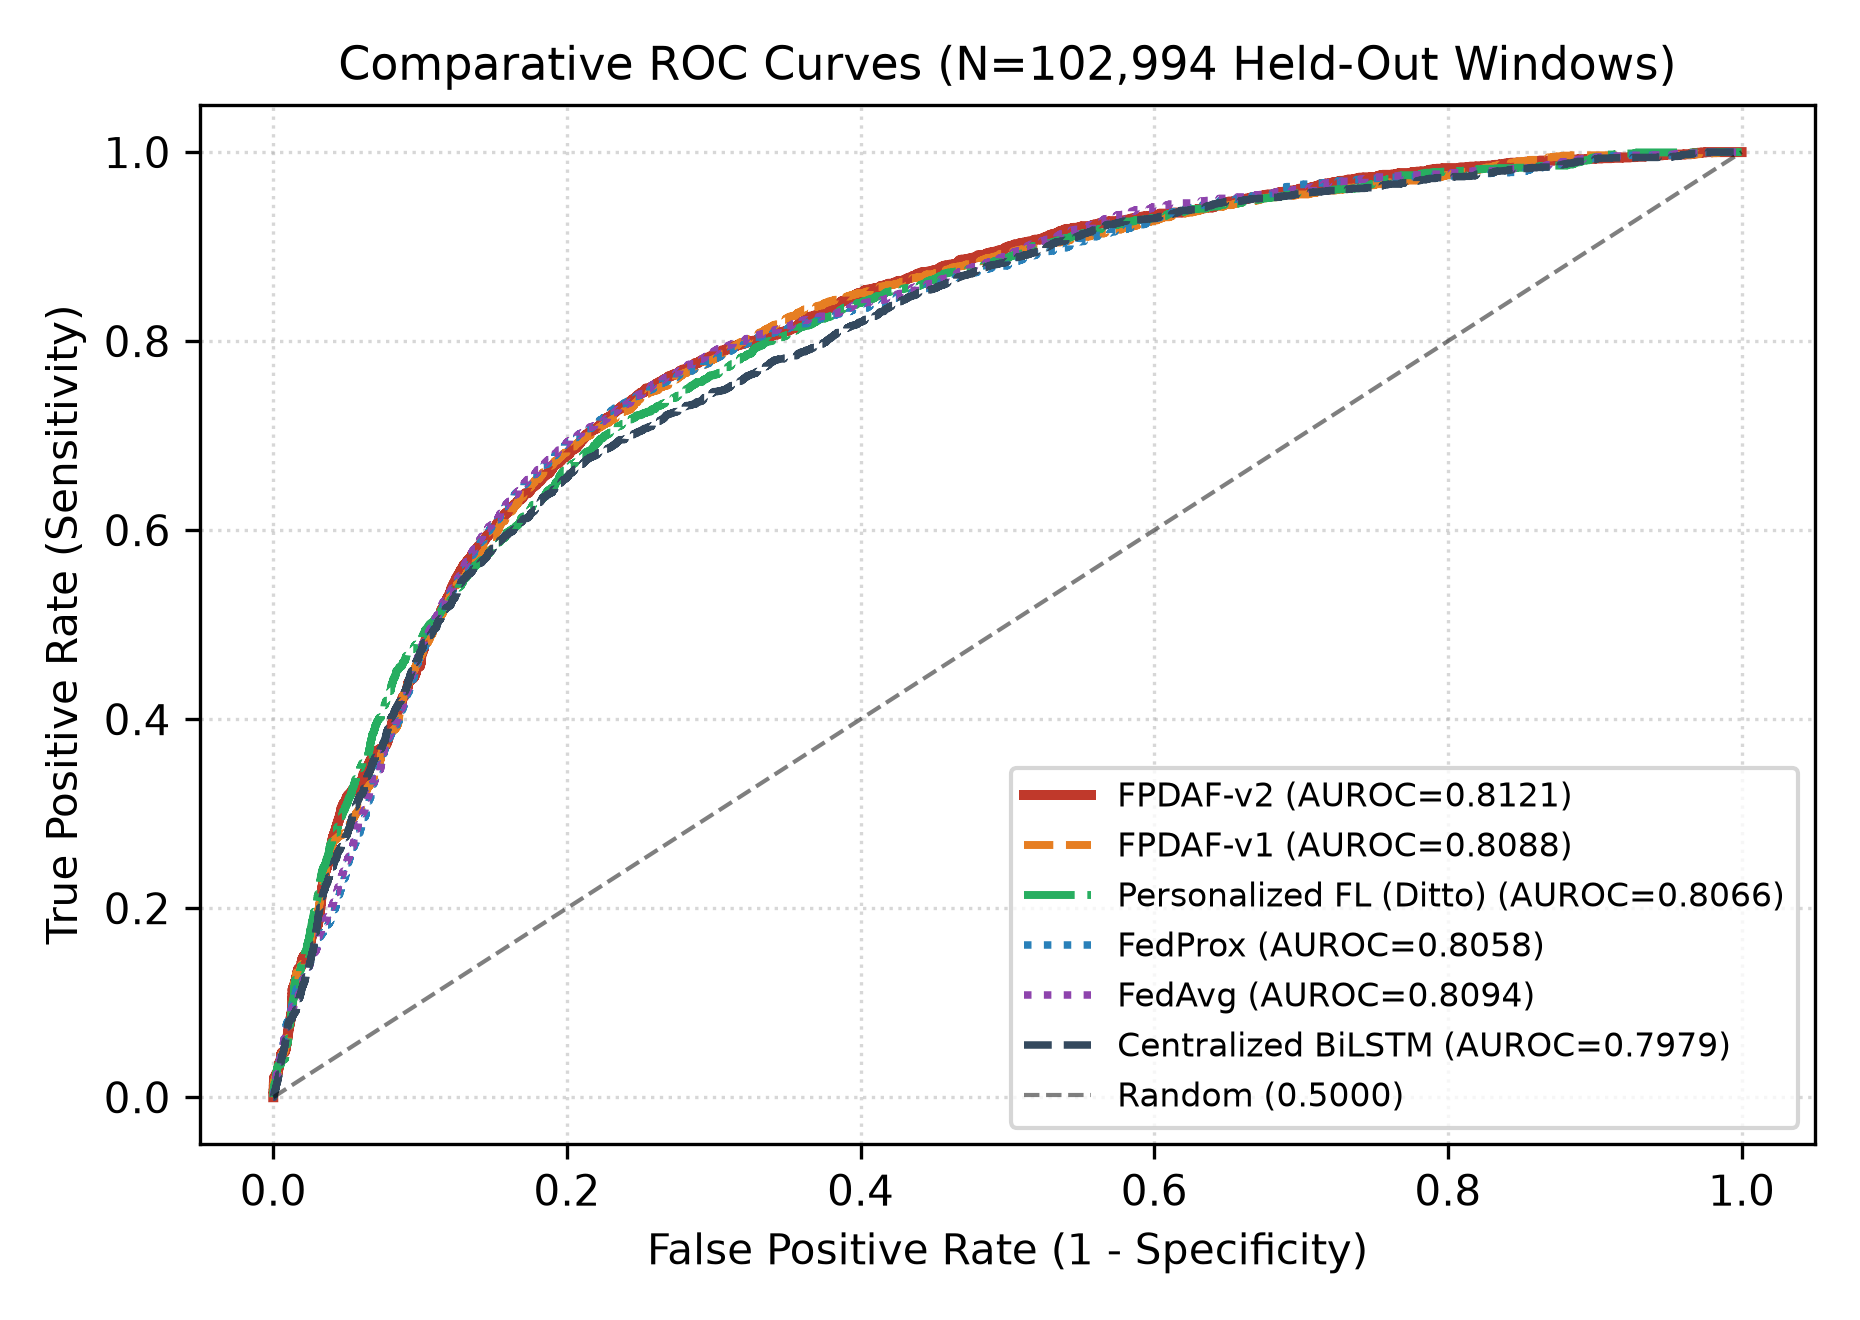
\includegraphics[width=0.38\textwidth]{images/federated_comparative_roc.png}\label{fig:empirical_roc}}
\hfill
\subfloat[Chronological AD-CUSUM Chart]{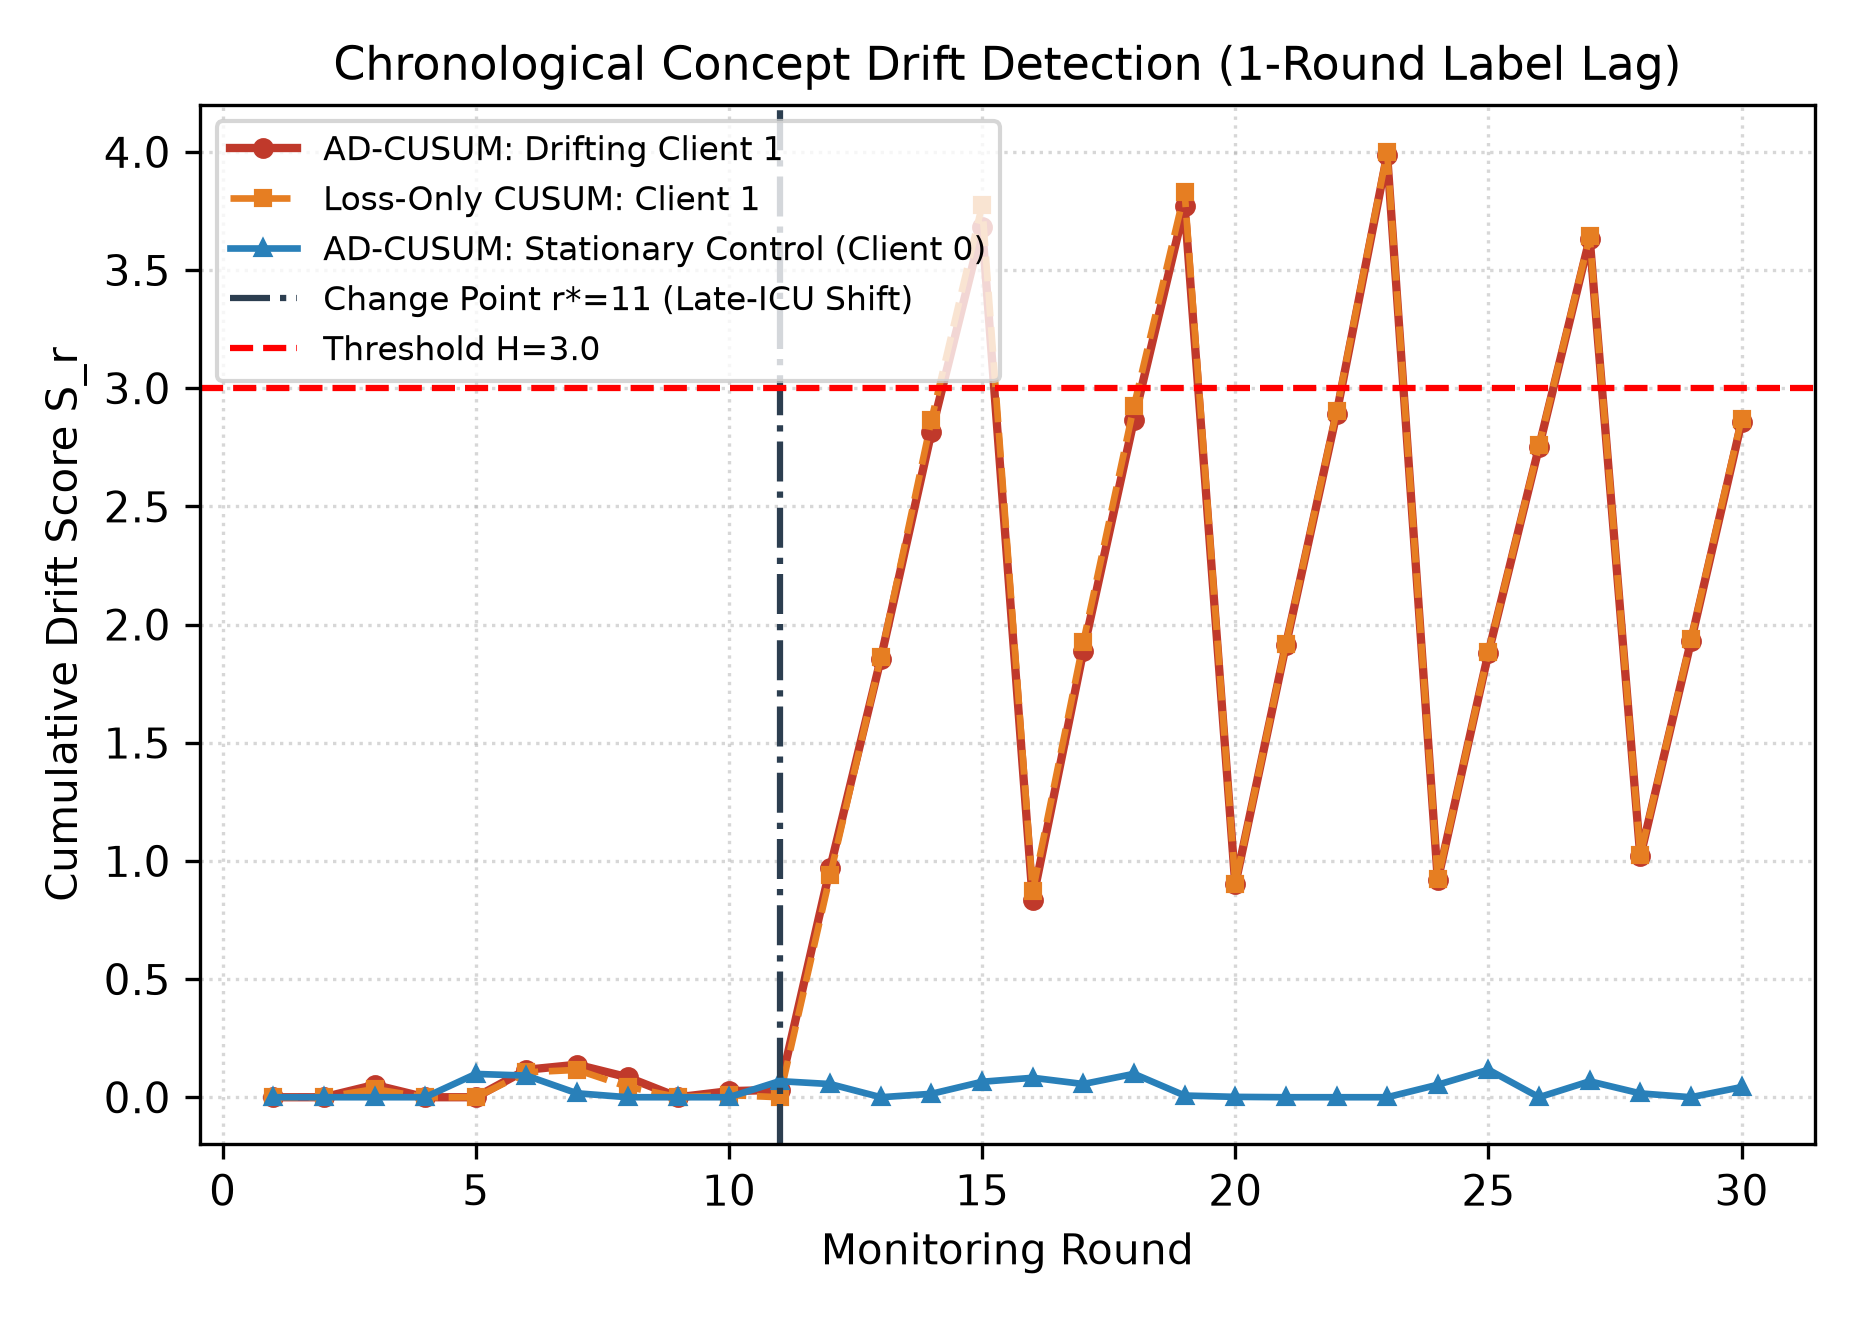
\includegraphics[width=0.38\textwidth]{images/cusum_drift_scores.png}\label{fig:empirical_drift}}
\par\vspace{1pt}
\subfloat[Validation Loss Convergence]{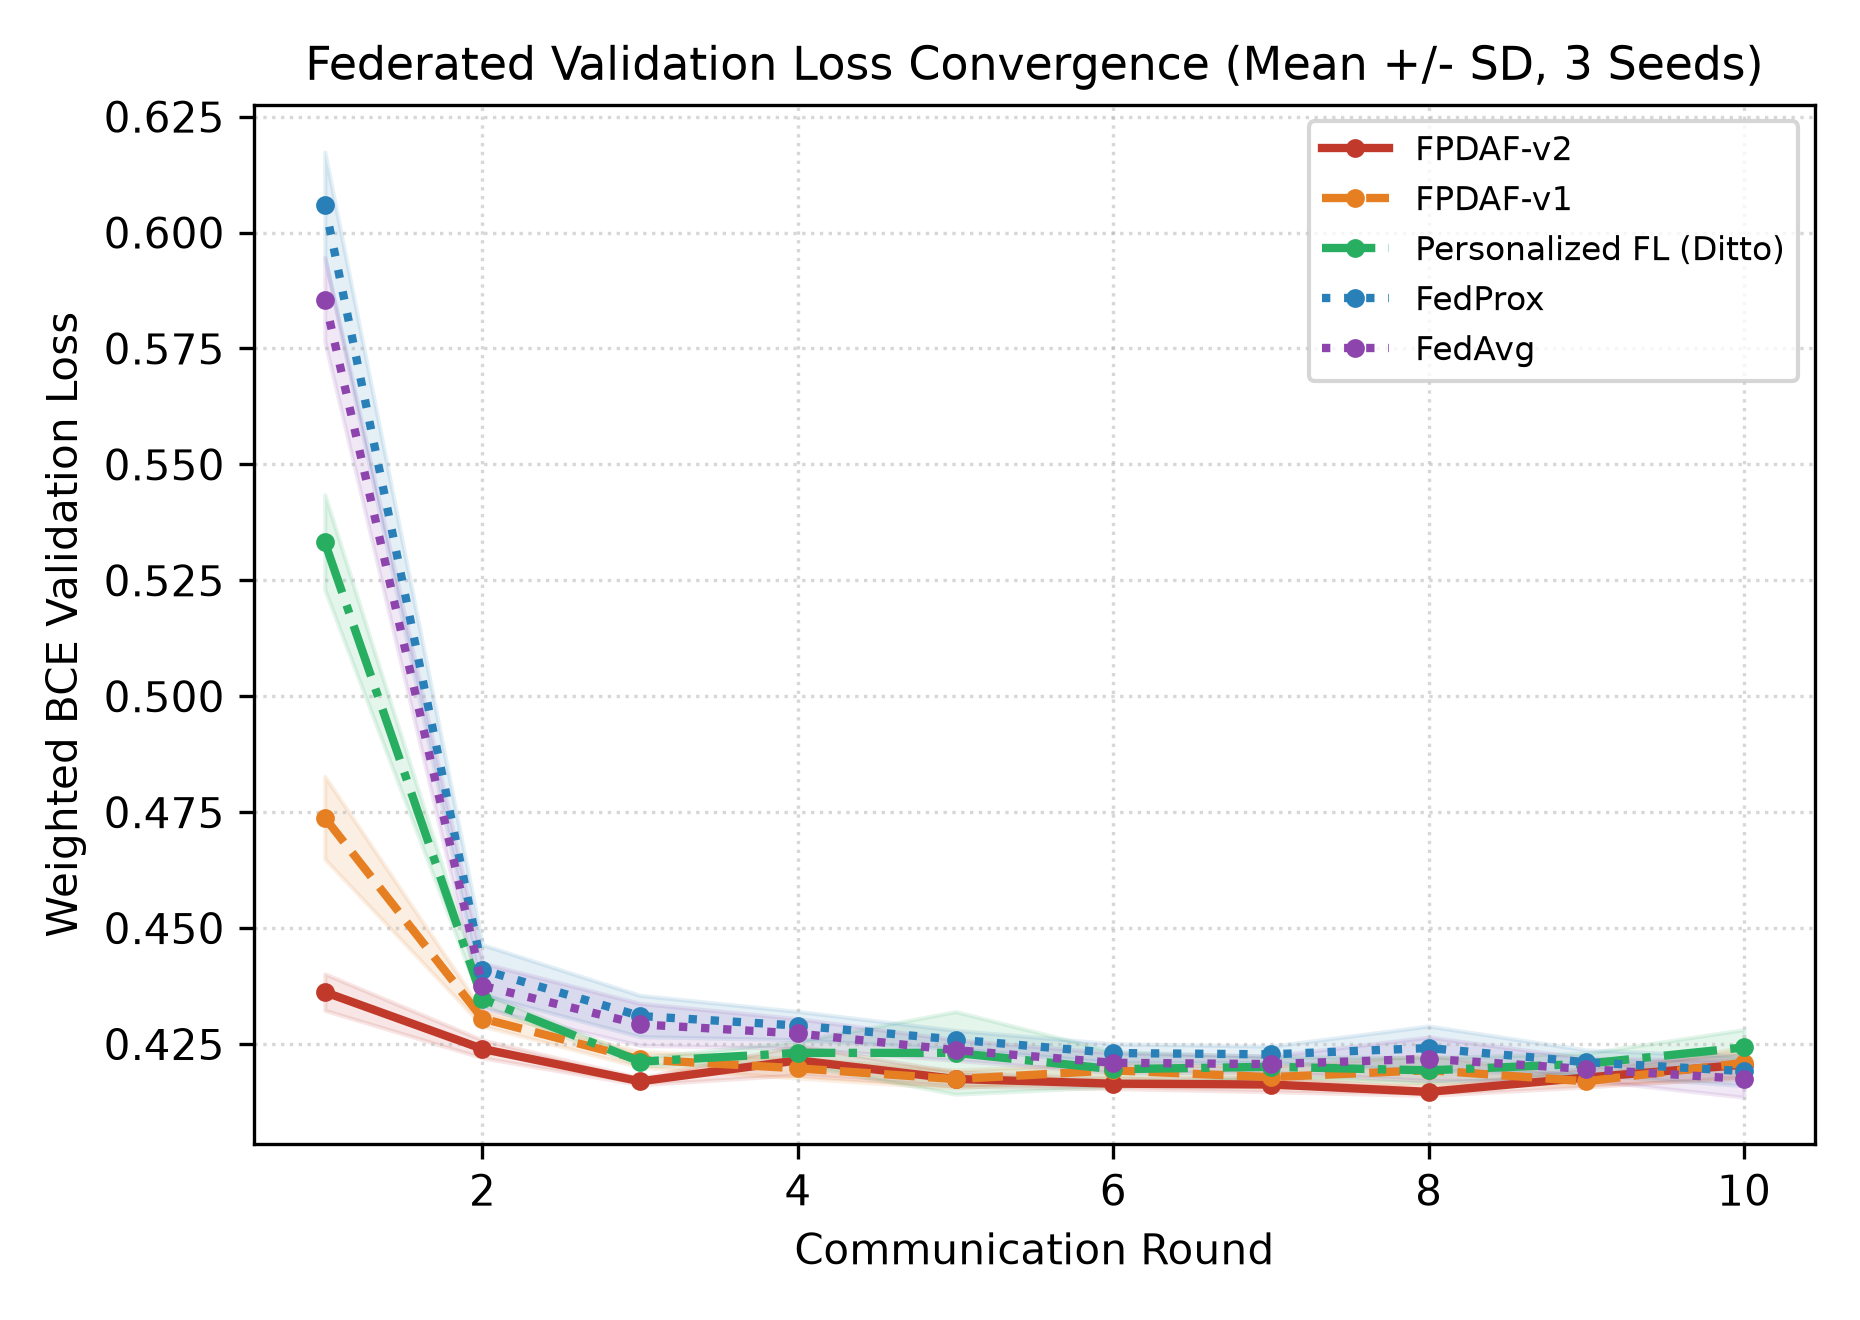
\includegraphics[width=0.38\textwidth]{images/federated_rounds_loss.png}\label{fig:empirical_loss}}
\hfill
\subfloat[24-Hour Temporal Attribution]{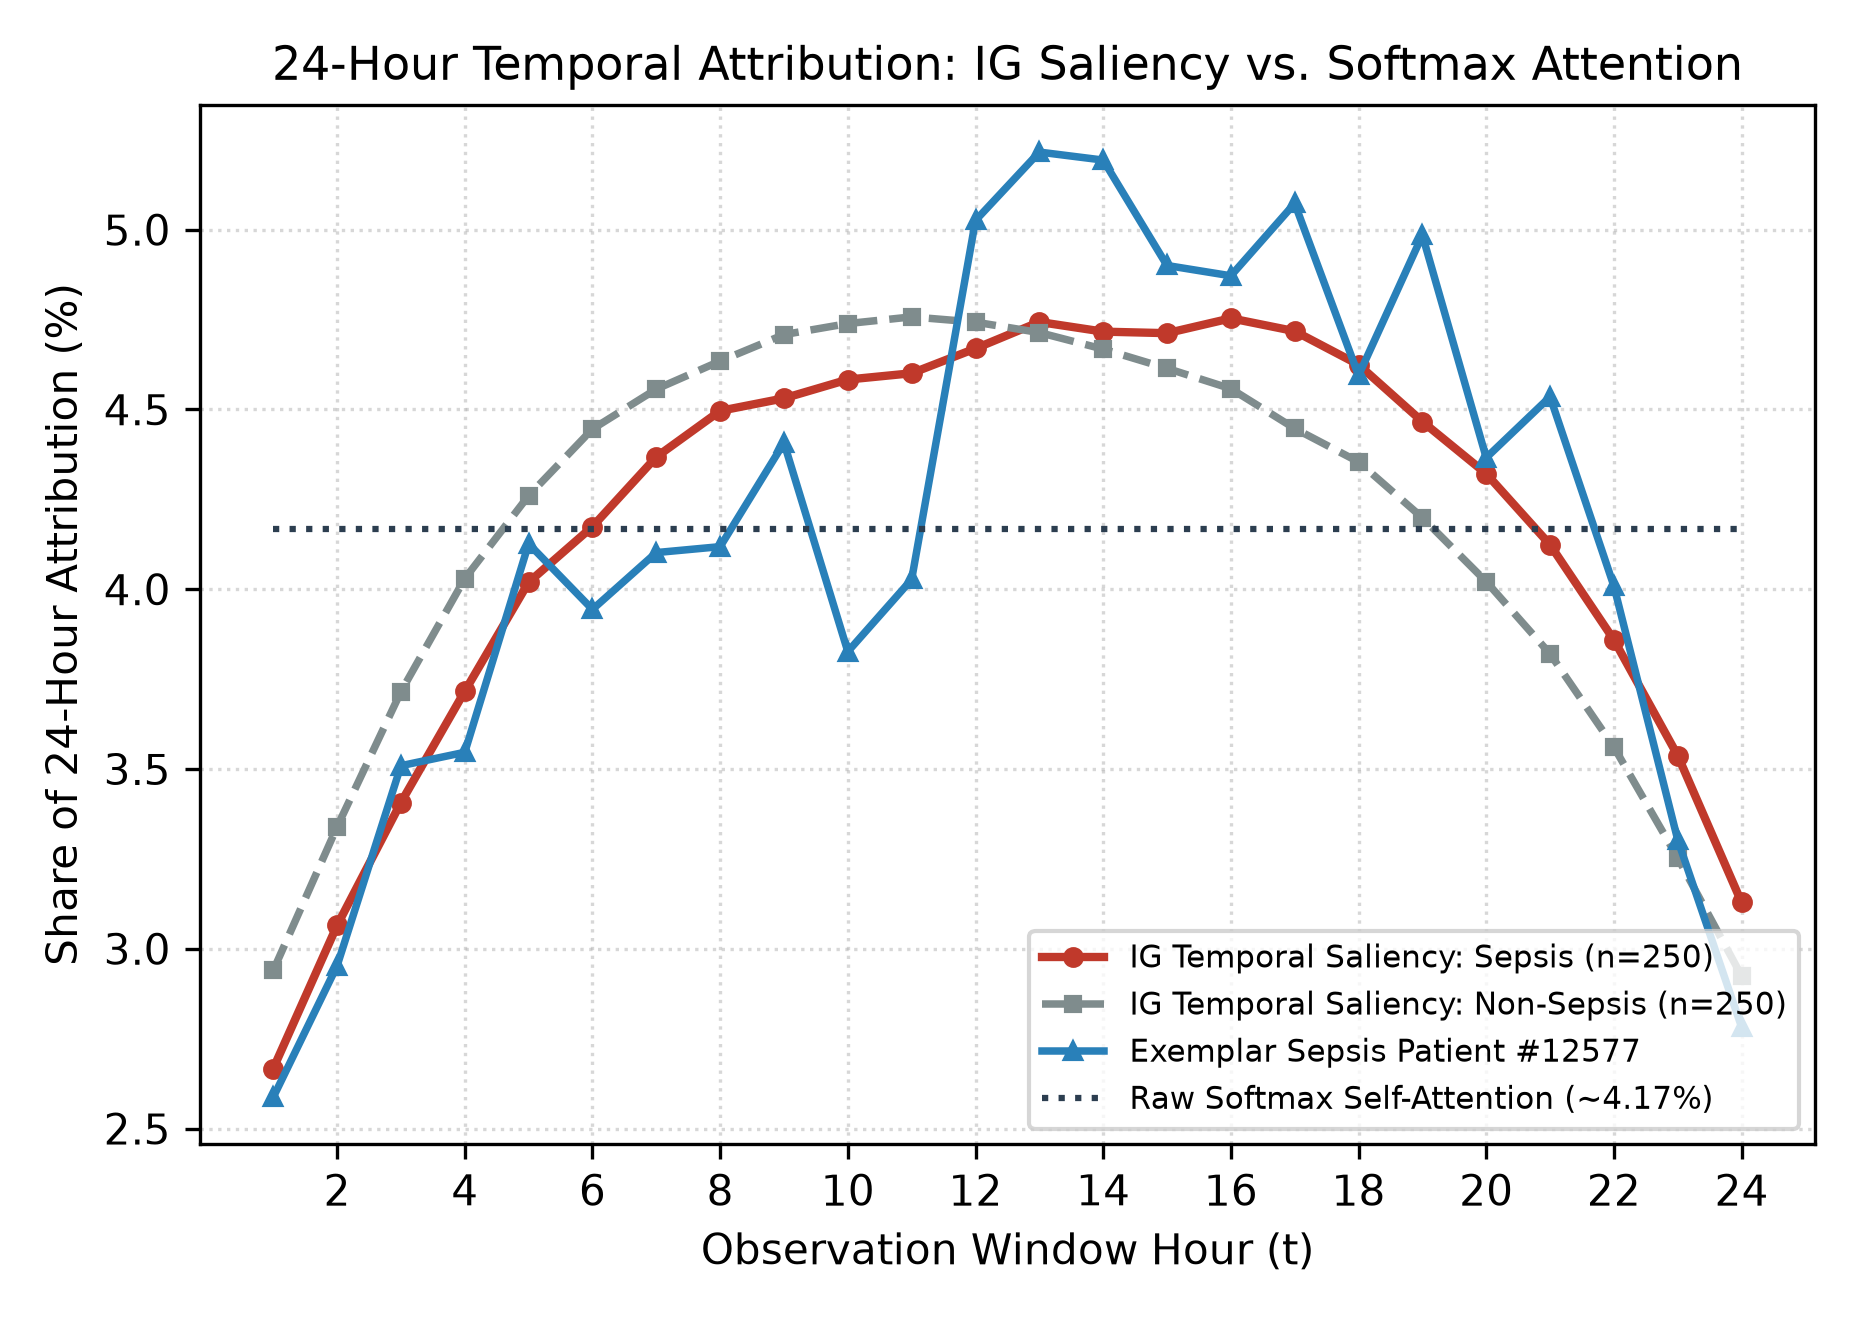
\includegraphics[width=0.38\textwidth]{images/temporal_attention_profile.png}\label{fig:temporal_attention}}
\caption{Audited evaluation ($N=102{,}994$ windows): (a) ROC curves; (b) 30-round drift chart ($r^*=11$, 1-round lag); (c) 3-seed validation loss ($\text{mean}\pm\text{SD}$); (d) 24-hour IG saliency vs.\ uniform softmax attention ($4.17\%$).}
\label{fig:combined}
\end{figure}

\begin{figure}[t]
\centering
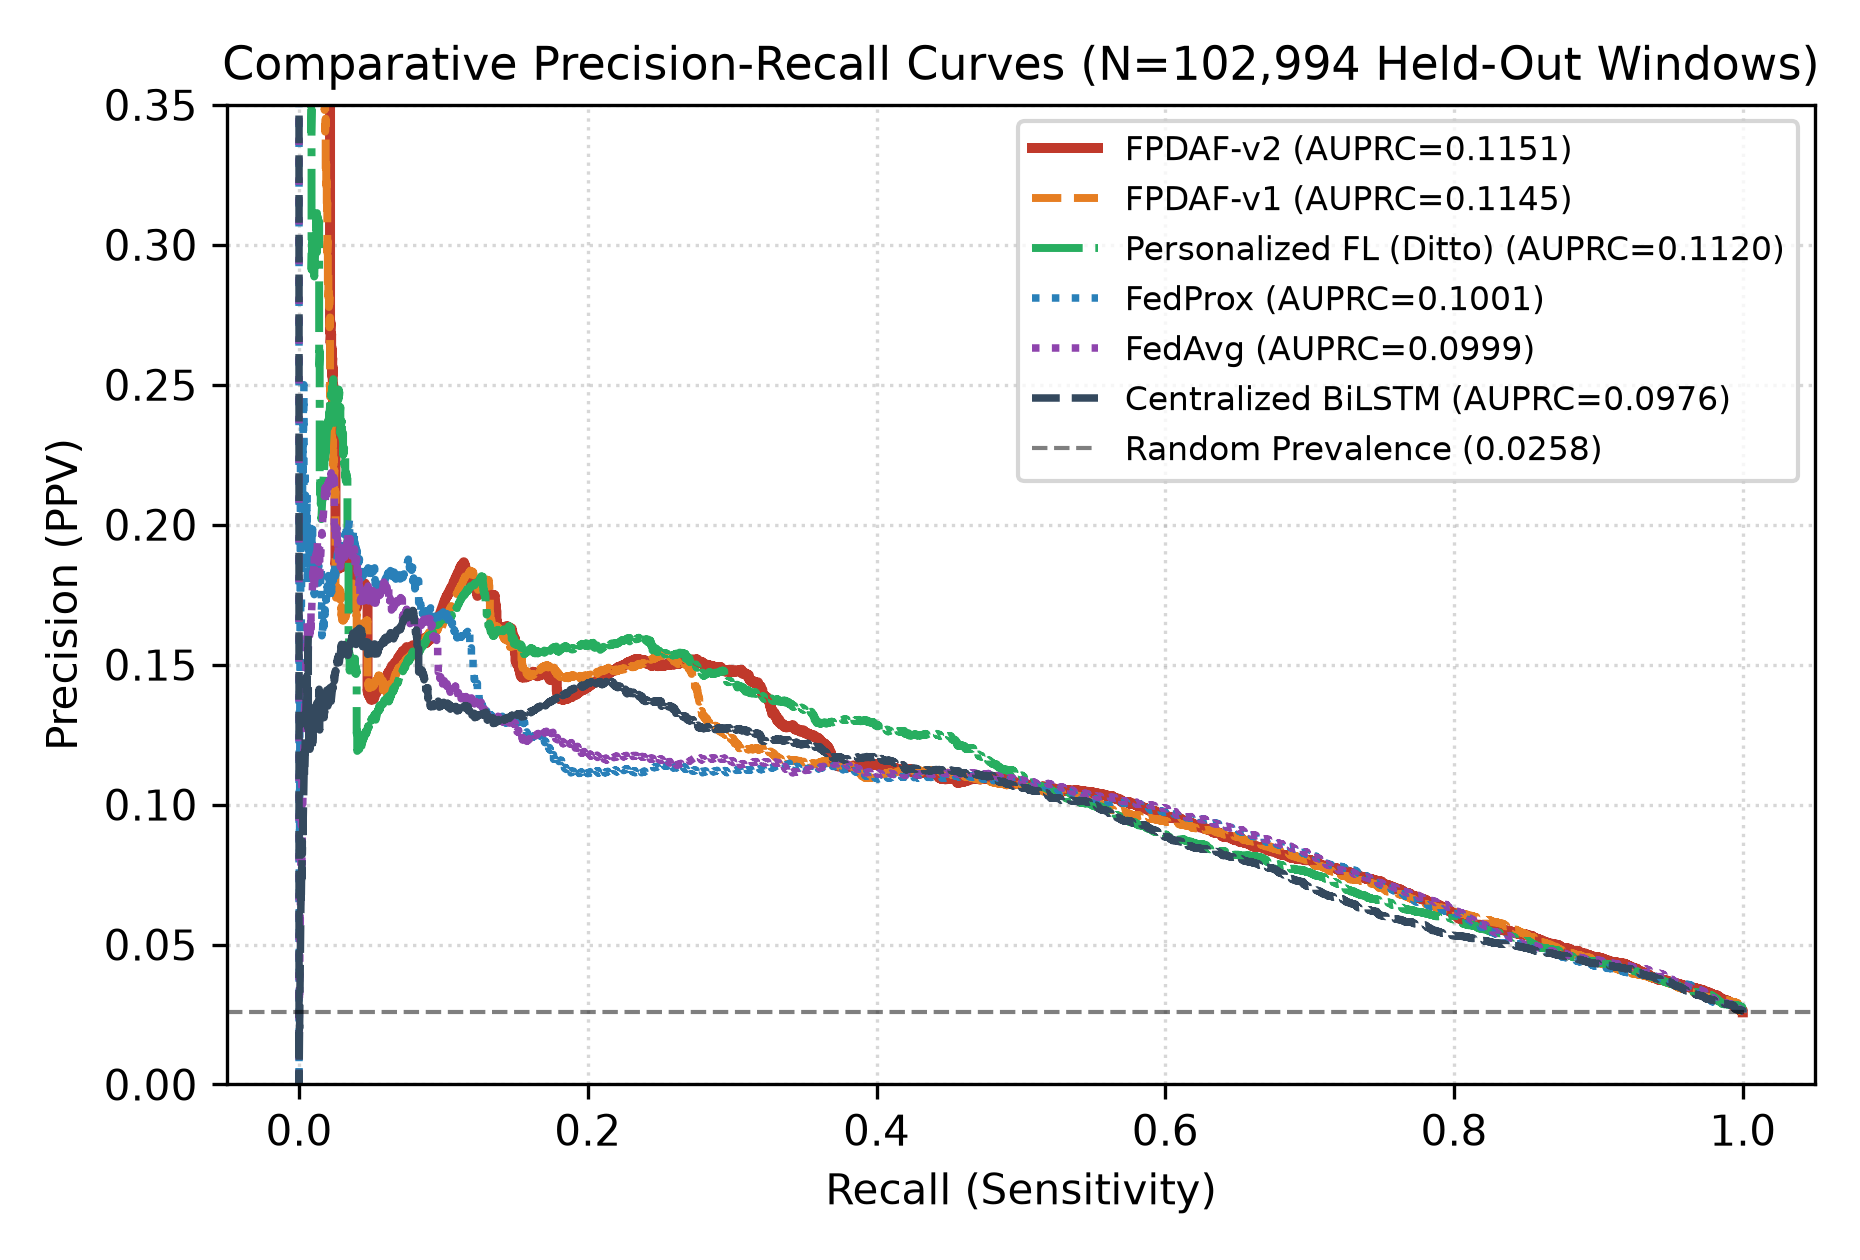
\includegraphics[width=0.44\textwidth]{images/federated_pr_curves.png}
\caption{Comparative Precision--Recall curves ($N=102{,}994$, $2.58\%$ prevalence floor).}
\label{fig:pr_curves}
\end{figure}

\section{Clinical Explainability and Computational Efficiency}

\subsection{Cohort Attribution, Stability, and Constrained Counterfactuals}

As mean-pooled multi-head self-attention weights stay relatively similar over the hours ($4.17\%$, in line with~\cite{9}), we combine attention visualization with Integrated Gradients~\cite{24} compared to zero baseline ($x'=0$, standardizing to the training mean) in $m=50$ steps over $500$ stratified test windows ($250$ sepsis, $250$ non-sepsis). Cohort temporal IG saliency peaks at Hour~16 ($4.75\%$) for sepsis vs.\ Hour~11 ($4.76\%$) for non-sepsis (Fig.~\ref{fig:combined}(d)). Across all $500$ windows, top mean absolute IG drivers are \texttt{ICULOS} ($0.1377$), \texttt{Chloride} ($0.0487$), \texttt{Resp} ($0.0407$), \texttt{Unit2} ($0.0400$), \texttt{HCO3} ($0.0342$), \texttt{HR} ($0.0284$), \texttt{EtCO2} ($0.0274$), \texttt{Potassium} ($0.0264$), and \texttt{Lactate} ($0.0232$), exhibiting high cosine perturbation stability ($0.9999$ at $\sigma=0.01$; $0.9970$ at $\sigma=0.05$).

To quantify non-causal input sensitivity across $n=100$ consecutive Client~1 true-positive alerts ($p\ge 0.49$), demographics and duration (\texttt{Age}, \texttt{Gender}, \texttt{Unit}, \texttt{HospAdmTime}, \texttt{ICULOS}) stay frozen over the final $6$~h while hemodynamic targets satisfy $\mathrm{MAP}=80\approx (\mathrm{SBP}+2\,\mathrm{DBP})/3$ ($\mathrm{SBP}=115$, $\mathrm{DBP}=65$~mmHg), optionally joined by $\mathrm{HR}=78$~bpm, $\mathrm{Resp}=16$/min, and $\mathrm{O}_2\mathrm{Sat}=98\%$. Across $100$ alerts, BP normalization changes risk by $-0.12$ percentage points (pp) mean (max drop $-3.92$~pp), and multi-vital normalization shifts risk by $-0.86$~pp mean (max $-9.93$~pp), showing shared reliance on metabolic and duration context. For true-positive Patient~$\#12577$ (Age $83.5$, HR $93$, SBP $113$, MAP $85$, DBP $79$, Resp $24$, $\mathrm{O}_2\mathrm{Sat}$ $94\%$, Lactate $3.10$~mmol/L, ICULOS $45$~h), IG ranks \texttt{Resp} ($22.3\%$), \texttt{ICULOS} ($9.5\%$), \texttt{Chloride} ($8.2\%$), and \texttt{Lactate} ($7.8\%$) peaking at Hour~13 ($5.22\%$); joint normalization shifts risk from $49.3\%$ to $47.5\%$ ($49.5\%$ BP-only), representing local statistical sensitivity rather than a clinical treatment effect.

\subsection{Communication Accounting and CPU Edge Profiling}

FPDAF-v2 comprises $232{,}962$ parameters ($941{,}132$~B serialized): a shared backbone ($224{,}641$~params, $906{,}200$~B) and a private head ($8{,}321$~params, $35{,}485$~B), with forward complexity $\mathcal{O}(Td+T^2d)$. Over 10 stationary rounds ($1\text{ MB}=10^6\text{ B}$), FPDAF-v2 exchanges $54.37$~MB ($27.19$~MB DL, $27.19$~MB UL), saving $2.06$~MB ($3.65\%$) vs.\ full-model FedAvg ($56.43$~MB). Raw wire volume exceeds non-attention BiLSTM FedAvg/Ditto ($39.23$~MB; $161{,}921$ params, $654{,}055$~B) due to attention capacity, whereas during drift rounds CSSP sends only a $1$-B flag, saving $1.81$~MB per client-round of backbone traffic (zero local XAI/probe traffic). CPU-only profiling on Apple~M4 ($10$~cores, $16$~GB RAM) measures $0.67\pm 0.02$~ms per window and $6.21\pm 0.10$~ms per $50$-bed batch.

\section{Discussion and Limitations}

Across $102{,}994$ held-out patient-disjoint windows, FPDAF-v2 improves discrimination ($0.8107$ AUROC, $0.1122$ AUPRC) and cross-seed stability ($\pm 0.0013$ AUROC SD) over all baselines, while quantifying alarm burden across validated operating modes ($80.98\%$ screening sensitivity at $5.83\%$ precision vs.\ $14.69\%$ F1-optimal precision at $30.89\%$ sensitivity). AD-CUSUM incurs $0.0\%$ false-positive cost stationarity penalty and recognizes temporal drift reliably for $H\in[1.5,4.0]$ while CSSP reduces Brier score Hospital~B error by $63.1\%$ and identifies when prior severe drift necessitates prevalence weighting or unfreezing. \textbf{Limitations:} (1) patients generated from a sole public dataset~\cite{23} without validation at an outside hospital; (2) labels are either pre-onset or post-onset hour; (3) past tensors contain within-admission backfill before the updated median training module; (4) static \texttt{pos\_weight=8.0} is poorly calibrated with prior shift $>4\times$; and (5) IG/Counterfactuals are associations rather than causal relations.

\section{Conclusion}

We presented FPDAF, unifying dual-phase cross-attention, AD-CUSUM drift detection, DDP-ERP distillation, and CSSP drift-only backbone freezing. Across $102{,}994$ held-out PhysioNet 2019 windows and three seeds, FPDAF-v2 attained $0.8107\pm 0.0013$ AUROC, $0.1122\pm 0.0021$ AUPRC, $0.0\%$ stationary FAR, $-1.81$~MB per CSSP drift round, and $0.67$~ms single-patient CPU latency; future work targets external hospital cohorts and prior-adaptive CSSP calibration.

\begin{thebibliography}{99}

\bibitem{1} Abdel-Sater, R., Hamza, A.B.: A federated large language model for long-term time series forecasting. In: Proc.\ ECAI, FAIA vol.\ 392, pp.\ 2452--2460 (2024). DOI: 10.3233/FAIA240772.
\bibitem{2} Jothimurugesan, E., Hsieh, K., Wang, J., Joshi, G., Gibbons, P.B.: Federated learning under distributed concept drift. In: Proc.\ AISTATS, PMLR vol.\ 206, pp.\ 5834--5853 (2023). DOI: 10.48550/arXiv.2206.00799.
\bibitem{3} Arivazhagan, M.G., Aggarwal, V., Singh, A.K., Choudhary, S.: Federated learning with personalization layers. arXiv:1912.00818 (2019). DOI: 10.48550/arXiv.1912.00818.
\bibitem{4} Yang, X., Wan, D., Han, G., Zhang, W., Tang, W.: Personalized federated learning with hierarchical reweighting for multi-center clinical prediction. Comput.\ Methods Programs Biomed.\ 271, 109015 (2025). DOI: 10.1016/j.cmpb.2025.109015.
\bibitem{5} D\"{u}sing, C., Cimiano, P.: Improving early sepsis onset prediction through federated learning. In: Artificial Intelligence for Biomedical Data, CCIS vol.\ 2696, pp.\ 3--16. Springer (2026). DOI: 10.1007/978-3-032-17216-7\_1.
\bibitem{6} Gupta, S., Torra, V.: Privacy-enhancing federated time-series forecasting: A microaggregation-based approach. In: Proc.\ SECRYPT, pp.\ 765--770 (2025). DOI: 10.5220/0013641100003979.
\bibitem{7} Casado, F.E., Lema, D., Criado, M.F., Iglesias, R., Regueiro, C.V., Barro, S.: Concept drift detection and adaptation for federated and continual learning. Multimed.\ Tools Appl.\ 81, 3397--3419 (2022). DOI: 10.1007/s11042-021-11219-x.
\bibitem{8} Kalakoti, R., N\~{o}mm, S., Bahsi, H.: Federated learning of explainable AI (FedXAI) for deep learning-based intrusion detection in IoT networks. Comput.\ Netw.\ 270, 111479 (2025). DOI: 10.1016/j.comnet.2025.111479.
\bibitem{9} Bari\'{c}, D., Fumi\'{c}, P., Horvati\'{c}, D., Lipic, T.: Benchmarking attention-based interpretability of deep learning in multivariate time series predictions. Entropy 23(2), 143 (2021). DOI: 10.3390/e23020143.
\bibitem{10} Ozyegen, O., Ilic, I., Cevik, M.: Evaluation of interpretability methods for multivariate time series forecasting. Appl.\ Intell.\ 52(5), 4727--4743 (2022). DOI: 10.1007/s10489-021-02662-2.
\bibitem{11} Lei, J., Zhai, J., Zhang, Y., Qi, J., Sun, C.: Supervised machine learning models for predicting sepsis-associated liver injury in patients with sepsis. J.\ Med.\ Internet Res.\ 27, e66733 (2025). DOI: 10.2196/66733.
\bibitem{12} Wei, H., Luo, Y., Xie, T., Yang, Y.: Federated learning with dual-end gradient correction and proxy-free self-distillation. IEEE Access 13, 162903--162914 (2025). DOI: 10.1109/ACCESS.2025.11165039.
\bibitem{13} Maher, M., Oun, O.F., Mesmeh, M.S., ElShawi, R.: FedForecaster: An automated federated learning approach for time-series forecasting. In: Proc.\ EDBT, pp.\ 867--873 (2025). DOI: 10.48786/EDBT.2025.70.
\bibitem{14} Maurya, A., Haripriya, R., Pandey, M., Choudhary, J., Singh, D.P., Solanki, S., Sharma, D.: Federated learning for privacy-preserving severity classification in healthcare. IEEE Access 13, 102339--102358 (2025). DOI: 10.1109/ACCESS.2025.3576135.
\bibitem{15} McMahan, H.B., Moore, E., Ramage, D., Hampson, S., Ag\"{u}era y Arcas, B.: Communication-efficient learning of deep networks from decentralized data. In: Proc.\ AISTATS, PMLR vol.\ 54, pp.\ 1273--1282 (2017).
\bibitem{16} Zhao, H., Sui, D., Wang, Y., Ma, L., Wang, L.: Privacy-preserving federated learning framework for multi-source EHR prognosis prediction. Sensors 25(8), 2374 (2025). DOI: 10.3390/s25082374.
\bibitem{17} Alam, M.U., Rahmani, R.: FedSepsis: A federated multi-modal deep learning IoMT application for early detection of sepsis. Sensors 23(2), 970 (2023). DOI: 10.3390/s23020970.
\bibitem{18} Tang, D., Yang, N., Li, Y., Zhu, Z., Jin, Z., Yuan, D.: Optimal look-back horizon for time series forecasting in federated learning. In: Proc.\ AAAI 40(30), pp.\ 25823--25830 (2026). DOI: 10.1609/aaai.v40i30.39781.
\bibitem{19} Wang, R., Bai, L., Rayhana, R., Liu, Z.: Personalized federated learning for buildings energy consumption forecasting. Energy Build.\ 323, 114762 (2024). DOI: 10.1016/j.enbuild.2024.114762.
\bibitem{20} Yang, X., Jung, J.P., Lu, J., Lim, K.W., Linguaglossa, L.: MVFL: Multivariate vertical federated learning for time-series forecasting. In: Proc.\ CNSM, pp.\ 1--7 (2025). DOI: 10.23919/CNSM67658.2025.11297529.
\bibitem{21} Singer, M., Deutschman, C.S., Seymour, C.W., et al.: The Third International Consensus Definitions for Sepsis and Septic Shock (Sepsis-3). JAMA 315(8), 801--810 (2016). DOI: 10.1001/jama.2016.0287.
\bibitem{22} Evans, L., Rhodes, A., Alhazzani, W., et al.: Surviving Sepsis Campaign: International guidelines for management of sepsis and septic shock 2021. Crit.\ Care Med.\ 49(11), e1063--e1143 (2021). DOI: 10.1097/CCM.0000000000005337.
\bibitem{23} Reyna, M.A., Josef, C.S., Jeter, R., et al.: Early prediction of sepsis from clinical data: The PhysioNet/CinC Challenge 2019. Crit.\ Care Med.\ 48(2), 210--217 (2020). DOI: 10.1097/CCM.0000000000004145.
\bibitem{24} Sundararajan, M., Taly, A., Yan, Q.: Axiomatic attribution for deep networks. In: Proc.\ ICML, PMLR vol.\ 70, pp.\ 3319--3328 (2017). DOI: 10.48550/arXiv.1703.01365.
\bibitem{25} Li, T., Sahu, A.K., Zaheer, M., Sanjabi, M., Talwalkar, A., Smith, V.: Federated optimization in heterogeneous networks. In: Proc.\ MLSys, vol.\ 2, pp.\ 429--450 (2020).
\bibitem{26} Li, T., Hu, S., Beirami, A., Smith, V.: Ditto: Fair and robust federated learning through personalization. In: Proc.\ ICML, PMLR vol.\ 139, pp.\ 6357--6368 (2021).

\end{thebibliography}

\end{document}
